% Options for packages loaded elsewhere
\PassOptionsToPackage{unicode}{hyperref}
\PassOptionsToPackage{hyphens}{url}
\PassOptionsToPackage{dvipsnames,svgnames,x11names}{xcolor}
%
\documentclass[
  letterpaper,
  DIV=11,
  numbers=noendperiod]{scrartcl}

\usepackage{amsmath,amssymb}
\usepackage{lmodern}
\usepackage{iftex}
\ifPDFTeX
  \usepackage[T1]{fontenc}
  \usepackage[utf8]{inputenc}
  \usepackage{textcomp} % provide euro and other symbols
\else % if luatex or xetex
  \usepackage{unicode-math}
  \defaultfontfeatures{Scale=MatchLowercase}
  \defaultfontfeatures[\rmfamily]{Ligatures=TeX,Scale=1}
\fi
% Use upquote if available, for straight quotes in verbatim environments
\IfFileExists{upquote.sty}{\usepackage{upquote}}{}
\IfFileExists{microtype.sty}{% use microtype if available
  \usepackage[]{microtype}
  \UseMicrotypeSet[protrusion]{basicmath} % disable protrusion for tt fonts
}{}
\makeatletter
\@ifundefined{KOMAClassName}{% if non-KOMA class
  \IfFileExists{parskip.sty}{%
    \usepackage{parskip}
  }{% else
    \setlength{\parindent}{0pt}
    \setlength{\parskip}{6pt plus 2pt minus 1pt}}
}{% if KOMA class
  \KOMAoptions{parskip=half}}
\makeatother
\usepackage{xcolor}
\setlength{\emergencystretch}{3em} % prevent overfull lines
\setcounter{secnumdepth}{-\maxdimen} % remove section numbering
% Make \paragraph and \subparagraph free-standing
\ifx\paragraph\undefined\else
  \let\oldparagraph\paragraph
  \renewcommand{\paragraph}[1]{\oldparagraph{#1}\mbox{}}
\fi
\ifx\subparagraph\undefined\else
  \let\oldsubparagraph\subparagraph
  \renewcommand{\subparagraph}[1]{\oldsubparagraph{#1}\mbox{}}
\fi


\providecommand{\tightlist}{%
  \setlength{\itemsep}{0pt}\setlength{\parskip}{0pt}}\usepackage{longtable,booktabs,array}
\usepackage{calc} % for calculating minipage widths
% Correct order of tables after \paragraph or \subparagraph
\usepackage{etoolbox}
\makeatletter
\patchcmd\longtable{\par}{\if@noskipsec\mbox{}\fi\par}{}{}
\makeatother
% Allow footnotes in longtable head/foot
\IfFileExists{footnotehyper.sty}{\usepackage{footnotehyper}}{\usepackage{footnote}}
\makesavenoteenv{longtable}
\usepackage{graphicx}
\makeatletter
\def\maxwidth{\ifdim\Gin@nat@width>\linewidth\linewidth\else\Gin@nat@width\fi}
\def\maxheight{\ifdim\Gin@nat@height>\textheight\textheight\else\Gin@nat@height\fi}
\makeatother
% Scale images if necessary, so that they will not overflow the page
% margins by default, and it is still possible to overwrite the defaults
% using explicit options in \includegraphics[width, height, ...]{}
\setkeys{Gin}{width=\maxwidth,height=\maxheight,keepaspectratio}
% Set default figure placement to htbp
\makeatletter
\def\fps@figure{htbp}
\makeatother

\KOMAoption{captions}{tableheading}
\makeatletter
\@ifpackageloaded{tcolorbox}{}{\usepackage[many]{tcolorbox}}
\@ifpackageloaded{fontawesome5}{}{\usepackage{fontawesome5}}
\definecolor{quarto-callout-color}{HTML}{909090}
\definecolor{quarto-callout-note-color}{HTML}{0758E5}
\definecolor{quarto-callout-important-color}{HTML}{CC1914}
\definecolor{quarto-callout-warning-color}{HTML}{EB9113}
\definecolor{quarto-callout-tip-color}{HTML}{00A047}
\definecolor{quarto-callout-caution-color}{HTML}{FC5300}
\definecolor{quarto-callout-color-frame}{HTML}{acacac}
\definecolor{quarto-callout-note-color-frame}{HTML}{4582ec}
\definecolor{quarto-callout-important-color-frame}{HTML}{d9534f}
\definecolor{quarto-callout-warning-color-frame}{HTML}{f0ad4e}
\definecolor{quarto-callout-tip-color-frame}{HTML}{02b875}
\definecolor{quarto-callout-caution-color-frame}{HTML}{fd7e14}
\makeatother
\makeatletter
\makeatother
\makeatletter
\makeatother
\makeatletter
\@ifpackageloaded{caption}{}{\usepackage{caption}}
\AtBeginDocument{%
\ifdefined\contentsname
  \renewcommand*\contentsname{Table of contents}
\else
  \newcommand\contentsname{Table of contents}
\fi
\ifdefined\listfigurename
  \renewcommand*\listfigurename{List of Figures}
\else
  \newcommand\listfigurename{List of Figures}
\fi
\ifdefined\listtablename
  \renewcommand*\listtablename{List of Tables}
\else
  \newcommand\listtablename{List of Tables}
\fi
\ifdefined\figurename
  \renewcommand*\figurename{Figure}
\else
  \newcommand\figurename{Figure}
\fi
\ifdefined\tablename
  \renewcommand*\tablename{Table}
\else
  \newcommand\tablename{Table}
\fi
}
\@ifpackageloaded{float}{}{\usepackage{float}}
\floatstyle{ruled}
\@ifundefined{c@chapter}{\newfloat{codelisting}{h}{lop}}{\newfloat{codelisting}{h}{lop}[chapter]}
\floatname{codelisting}{Listing}
\newcommand*\listoflistings{\listof{codelisting}{List of Listings}}
\makeatother
\makeatletter
\@ifpackageloaded{caption}{}{\usepackage{caption}}
\@ifpackageloaded{subcaption}{}{\usepackage{subcaption}}
\makeatother
\makeatletter
\@ifpackageloaded{tcolorbox}{}{\usepackage[many]{tcolorbox}}
\makeatother
\makeatletter
\@ifundefined{shadecolor}{\definecolor{shadecolor}{rgb}{.97, .97, .97}}
\makeatother
\makeatletter
\makeatother
\ifLuaTeX
  \usepackage{selnolig}  % disable illegal ligatures
\fi
\IfFileExists{bookmark.sty}{\usepackage{bookmark}}{\usepackage{hyperref}}
\IfFileExists{xurl.sty}{\usepackage{xurl}}{} % add URL line breaks if available
\urlstyle{same} % disable monospaced font for URLs
\hypersetup{
  pdftitle={Thoughts on Rates: a Chart Pack, Fall 2022},
  pdfauthor={Art Steinmetz},
  colorlinks=true,
  linkcolor={blue},
  filecolor={Maroon},
  citecolor={Blue},
  urlcolor={Blue},
  pdfcreator={LaTeX via pandoc}}

\title{Thoughts on Rates: a Chart Pack, Fall 2022}
\author{Art Steinmetz}
\date{}

\begin{document}
\maketitle
\ifdefined\Shaded\renewenvironment{Shaded}{\begin{tcolorbox}[borderline west={3pt}{0pt}{shadecolor}, enhanced, boxrule=0pt, interior hidden, breakable, sharp corners, frame hidden]}{\end{tcolorbox}}\fi

\hypertarget{part-two-much-more-pain}{%
\section{Part Two: Much More Pain}\label{part-two-much-more-pain}}

\hypertarget{what-will-happen.}{%
\subsection{What Will Happen.}\label{what-will-happen.}}

One thing that makes pundits boring is their endless explanations of the
past (Oops, guilty) with scant conviction on what the future holds. So
let's get to that. ``They'' will tell you that the yield curve is
inverted because 10s are lower than 2s. ``They'' are wrong. I stick to
my prediction of the Spring. Bond markets will continue to suffer until
the Funds rate climbs above the 10-year yield. See
\href{https://www.linkedin.com/posts/asteinmetz_markets-activity-6914653620307140610-wgYi}{my
post from March 2022 for the rationale}. It has aged pretty well.

\begin{tcolorbox}[enhanced jigsaw, arc=.35mm, toprule=.15mm, breakable, colframe=quarto-callout-note-color-frame, leftrule=.75mm, left=2mm, opacityback=0, bottomrule=.15mm, rightrule=.15mm, colback=white]
\emph{To be clear, the long end has a long way to go and the funds rate
even longer.}~

\emph{The market must be shocked and awed by the level of the funds rate
or the inflation rate will remain stubbornly high.}
\end{tcolorbox}

\ldots{} and \ldots{}

\begin{tcolorbox}[enhanced jigsaw, arc=.35mm, toprule=.15mm, breakable, colframe=quarto-callout-note-color-frame, leftrule=.75mm, left=2mm, opacityback=0, bottomrule=.15mm, rightrule=.15mm, colback=white]
\emph{In the ``typical'' tightening cycle we find stocks enter a brief
correction when the weathervane at the top of the Fed swings around to
tightening but continue on their merry way after a month or so.~Only
when the hikes truly bite - inversion happens, a recession is triggered
- do we we see the market crap out.~This time I see a long winter ahead,
without much of a respite during the tightening phase.}
\end{tcolorbox}

My dodge is I don't predict what that level will be. I have seriously
heard people say things like ``Well, after the next hike we'll be
there.'' They forget that the bond market can move too, and it will. As
James Makintosh
\href{https://www.wsj.com/articles/markets-keep-making-the-same-mistake-about-inflation-11663163494?mod=markets_lead_pos6}{writes
in the Wall Street Journal}, just as the Fed is behind the curve, so are
investors. Hindsight bias means people are still unappreciative of how
high rates can go.

One of the contradictions of market forecasters and curve shape is that
when the curve inverts it predicts a recession and a recession is bad
for the markets. My friends at Deutsche Bank produce a very nice probit
model based on the yield curve that shows the probability of recession.
As a trader, I don't care. The problem is macroeconomic data is a
lagging indicator of what markets do and so is useless for market
forecasting. The forecasters' logic is circular.

\textbf{NOT TRUE:}

\textbf{Markets} \emph{--predict-\textgreater{}} \textbf{Economy}
\emph{--predict-\textgreater{}} \textbf{Markets}

\hypertarget{what-to-do.}{%
\subsection{What To Do.}\label{what-to-do.}}

The nice thing about Fed Funds vs.~long rates is it signals a bond
market bottom. We don't have to agonize over whether, several years from
now, the NBER will label the current moment a recession.

So I have a clear view that when the ``true'' inversion happens the bond
market will have bottomed and it's time to get in. The same is not true
for stocks, as I said in my last note. So, avoid stocks. Cash is king
but the next trade is to buy bonds. In the chart below, the green zone
shows the ``true'' inversion periods and thus the ``buy zone.'' How
reasonable is that proposition?

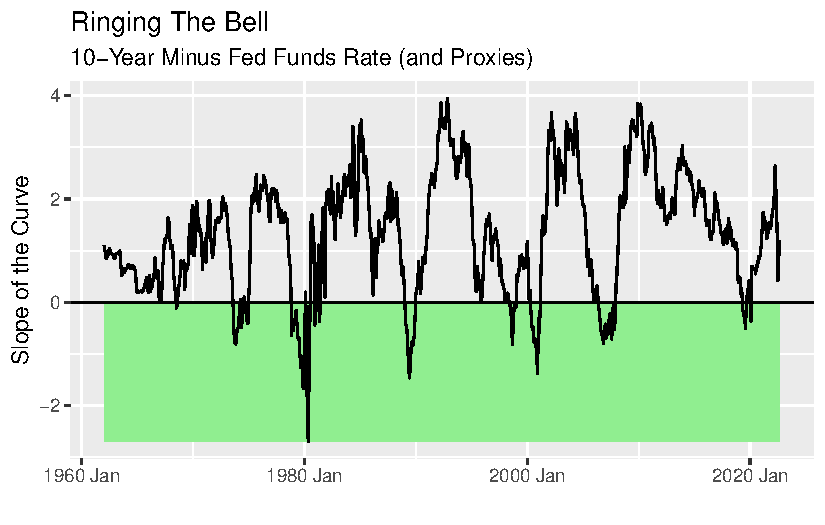
\includegraphics{thoughts_on_rates_pt2_files/figure-pdf/ring_the_bell-1.pdf}

Above we see the inversion periods. What happens to bond yields when we
enter those zones? The economy truly slows down, inflation abates and
Treasury bond prices start to rise again. That is evident from the chart
below.

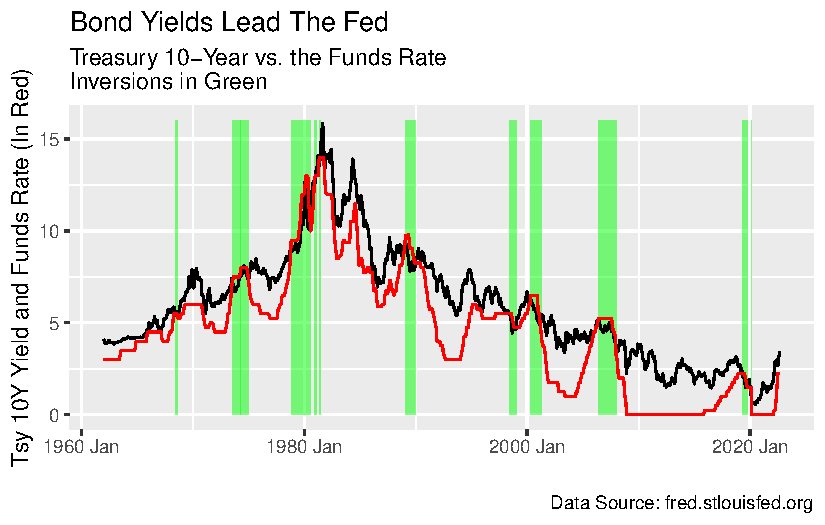
\includegraphics{thoughts_on_rates_pt2_files/figure-pdf/yeilds_lead_fed-1.pdf}

The ``buy'' signal is not as clear-cut as we would like. The timing
could be tricky and we see at least one false signal in the late 90s. I
have some optimism that we will get a good signal this time. Why?
Inflation is stubborn and the level of the Funds Rate we will have to
reach to bring it down is going to be ``pretty high.'' The consequence
of being so far behind means the Fed will have to overshoot to show it
means business. This suggests the slowdown will be pronounced. Bond
yields will start their rally from levels we haven't seen since the
naughts. Remember when a 5\% bond yield seemed normal? It will again,
soon.

What would have happened had the Fed started raising rates a year ago?
Could we have seen only a modest rise in long rates, like we did in the
last two tightening cycles? We'll never know. Are we doomed to see a
reversal of the 40-year rally in bonds. This could happen if the Fed
response is insufficiently vigorous, as happened in the CPI run up after
the first oil shock in 1973.

So we have a time, give or take, to buy bonds. Unfortunately for stocks,
when this curve shape occurs (and not before) it shows investors finally
are resigned to a real recession beginning. This is when it gets tough
for company earnings. The bottom for equities will come later.

In my next note we'll try to come up with a trading rule around when to
buy bonds and how long to hold them. In the meantime, remember, cash is
king.



\end{document}
